\documentclass[]{article}
\usepackage{lmodern}
\usepackage{amssymb,amsmath}
\usepackage{ifxetex,ifluatex}
\usepackage{fixltx2e} % provides \textsubscript
\ifnum 0\ifxetex 1\fi\ifluatex 1\fi=0 % if pdftex
  \usepackage[T1]{fontenc}
  \usepackage[utf8]{inputenc}
\else % if luatex or xelatex
  \ifxetex
    \usepackage{mathspec}
  \else
    \usepackage{fontspec}
  \fi
  \defaultfontfeatures{Ligatures=TeX,Scale=MatchLowercase}
\fi
% use upquote if available, for straight quotes in verbatim environments
\IfFileExists{upquote.sty}{\usepackage{upquote}}{}
% use microtype if available
\IfFileExists{microtype.sty}{%
\usepackage{microtype}
\UseMicrotypeSet[protrusion]{basicmath} % disable protrusion for tt fonts
}{}
\usepackage[margin=1in]{geometry}
\usepackage{hyperref}
\hypersetup{unicode=true,
            pdftitle={Homework 6},
            pdfauthor={Emorie Beck},
            pdfborder={0 0 0},
            breaklinks=true}
\urlstyle{same}  % don't use monospace font for urls
\usepackage{color}
\usepackage{fancyvrb}
\newcommand{\VerbBar}{|}
\newcommand{\VERB}{\Verb[commandchars=\\\{\}]}
\DefineVerbatimEnvironment{Highlighting}{Verbatim}{commandchars=\\\{\}}
% Add ',fontsize=\small' for more characters per line
\usepackage{framed}
\definecolor{shadecolor}{RGB}{248,248,248}
\newenvironment{Shaded}{\begin{snugshade}}{\end{snugshade}}
\newcommand{\KeywordTok}[1]{\textcolor[rgb]{0.13,0.29,0.53}{\textbf{#1}}}
\newcommand{\DataTypeTok}[1]{\textcolor[rgb]{0.13,0.29,0.53}{#1}}
\newcommand{\DecValTok}[1]{\textcolor[rgb]{0.00,0.00,0.81}{#1}}
\newcommand{\BaseNTok}[1]{\textcolor[rgb]{0.00,0.00,0.81}{#1}}
\newcommand{\FloatTok}[1]{\textcolor[rgb]{0.00,0.00,0.81}{#1}}
\newcommand{\ConstantTok}[1]{\textcolor[rgb]{0.00,0.00,0.00}{#1}}
\newcommand{\CharTok}[1]{\textcolor[rgb]{0.31,0.60,0.02}{#1}}
\newcommand{\SpecialCharTok}[1]{\textcolor[rgb]{0.00,0.00,0.00}{#1}}
\newcommand{\StringTok}[1]{\textcolor[rgb]{0.31,0.60,0.02}{#1}}
\newcommand{\VerbatimStringTok}[1]{\textcolor[rgb]{0.31,0.60,0.02}{#1}}
\newcommand{\SpecialStringTok}[1]{\textcolor[rgb]{0.31,0.60,0.02}{#1}}
\newcommand{\ImportTok}[1]{#1}
\newcommand{\CommentTok}[1]{\textcolor[rgb]{0.56,0.35,0.01}{\textit{#1}}}
\newcommand{\DocumentationTok}[1]{\textcolor[rgb]{0.56,0.35,0.01}{\textbf{\textit{#1}}}}
\newcommand{\AnnotationTok}[1]{\textcolor[rgb]{0.56,0.35,0.01}{\textbf{\textit{#1}}}}
\newcommand{\CommentVarTok}[1]{\textcolor[rgb]{0.56,0.35,0.01}{\textbf{\textit{#1}}}}
\newcommand{\OtherTok}[1]{\textcolor[rgb]{0.56,0.35,0.01}{#1}}
\newcommand{\FunctionTok}[1]{\textcolor[rgb]{0.00,0.00,0.00}{#1}}
\newcommand{\VariableTok}[1]{\textcolor[rgb]{0.00,0.00,0.00}{#1}}
\newcommand{\ControlFlowTok}[1]{\textcolor[rgb]{0.13,0.29,0.53}{\textbf{#1}}}
\newcommand{\OperatorTok}[1]{\textcolor[rgb]{0.81,0.36,0.00}{\textbf{#1}}}
\newcommand{\BuiltInTok}[1]{#1}
\newcommand{\ExtensionTok}[1]{#1}
\newcommand{\PreprocessorTok}[1]{\textcolor[rgb]{0.56,0.35,0.01}{\textit{#1}}}
\newcommand{\AttributeTok}[1]{\textcolor[rgb]{0.77,0.63,0.00}{#1}}
\newcommand{\RegionMarkerTok}[1]{#1}
\newcommand{\InformationTok}[1]{\textcolor[rgb]{0.56,0.35,0.01}{\textbf{\textit{#1}}}}
\newcommand{\WarningTok}[1]{\textcolor[rgb]{0.56,0.35,0.01}{\textbf{\textit{#1}}}}
\newcommand{\AlertTok}[1]{\textcolor[rgb]{0.94,0.16,0.16}{#1}}
\newcommand{\ErrorTok}[1]{\textcolor[rgb]{0.64,0.00,0.00}{\textbf{#1}}}
\newcommand{\NormalTok}[1]{#1}
\usepackage{graphicx,grffile}
\makeatletter
\def\maxwidth{\ifdim\Gin@nat@width>\linewidth\linewidth\else\Gin@nat@width\fi}
\def\maxheight{\ifdim\Gin@nat@height>\textheight\textheight\else\Gin@nat@height\fi}
\makeatother
% Scale images if necessary, so that they will not overflow the page
% margins by default, and it is still possible to overwrite the defaults
% using explicit options in \includegraphics[width, height, ...]{}
\setkeys{Gin}{width=\maxwidth,height=\maxheight,keepaspectratio}
\IfFileExists{parskip.sty}{%
\usepackage{parskip}
}{% else
\setlength{\parindent}{0pt}
\setlength{\parskip}{6pt plus 2pt minus 1pt}
}
\setlength{\emergencystretch}{3em}  % prevent overfull lines
\providecommand{\tightlist}{%
  \setlength{\itemsep}{0pt}\setlength{\parskip}{0pt}}
\setcounter{secnumdepth}{0}
% Redefines (sub)paragraphs to behave more like sections
\ifx\paragraph\undefined\else
\let\oldparagraph\paragraph
\renewcommand{\paragraph}[1]{\oldparagraph{#1}\mbox{}}
\fi
\ifx\subparagraph\undefined\else
\let\oldsubparagraph\subparagraph
\renewcommand{\subparagraph}[1]{\oldsubparagraph{#1}\mbox{}}
\fi

%%% Use protect on footnotes to avoid problems with footnotes in titles
\let\rmarkdownfootnote\footnote%
\def\footnote{\protect\rmarkdownfootnote}

%%% Change title format to be more compact
\usepackage{titling}

% Create subtitle command for use in maketitle
\newcommand{\subtitle}[1]{
  \posttitle{
    \begin{center}\large#1\end{center}
    }
}

\setlength{\droptitle}{-2em}
  \title{Homework 6}
  \pretitle{\vspace{\droptitle}\centering\huge}
  \posttitle{\par}
\subtitle{Psych 5068}
  \author{Emorie Beck}
  \preauthor{\centering\large\emph}
  \postauthor{\par}
  \predate{\centering\large\emph}
  \postdate{\par}
  \date{\today}

\usepackage{fancyhdr}
\usepackage{array}
\usepackage{longtable}
\usepackage{lscape}
\newcommand{\blandscape}{\begin{landscape}}
\newcommand{\elandscape}{\end{landscape}}
\usepackage{dcolumn}
\usepackage{bbm}
\usepackage{threeparttable}
\usepackage{booktabs}
\usepackage{expex}
\usepackage{rotating, graphicx}
\usepackage{tabulary}
\usepackage{algorithm}
\usepackage{multirow}
\usepackage{colortbl}
\usepackage{longtable}
\usepackage{array}
\usepackage{multirow}
\usepackage[table]{xcolor}
\usepackage{wrapfig}
\usepackage{float}
\usepackage{pdflscape}
\usepackage{tabu}
\usepackage{threeparttable}
\usepackage{booktabs}
\usepackage{longtable}
\usepackage{array}
\usepackage{multirow}
\usepackage[table]{xcolor}
\usepackage{wrapfig}
\usepackage{float}
\usepackage{colortbl}
\usepackage{pdflscape}
\usepackage{tabu}
\usepackage{threeparttable}
\usepackage[normalem]{ulem}

\begin{document}
\maketitle

{
\setcounter{tocdepth}{2}
\tableofcontents
}
For this assignment, you will extend our analyses of the Curran reading
data (Curran\_New\_Trimmed.csv).

\section{Workspace}\label{workspace}

\subsection{Packages}\label{packages}

\begin{Shaded}
\begin{Highlighting}[]
\KeywordTok{library}\NormalTok{(psych)}
\KeywordTok{library}\NormalTok{(lme4)}
\KeywordTok{library}\NormalTok{(knitr)}
\KeywordTok{library}\NormalTok{(qqplotr)}
\KeywordTok{library}\NormalTok{(influence.ME)}
\KeywordTok{library}\NormalTok{(HLMdiag)}
\KeywordTok{library}\NormalTok{(multcomp)}
\KeywordTok{library}\NormalTok{(kableExtra)}
\KeywordTok{library}\NormalTok{(plyr)}
\KeywordTok{library}\NormalTok{(tidyverse)}
\end{Highlighting}
\end{Shaded}

\subsection{Data}\label{data}

\begin{Shaded}
\begin{Highlighting}[]
\NormalTok{data_url <-}\StringTok{ "https://raw.githubusercontent.com/emoriebeck/homeworks/master/homework6/Curran_New_Trimmed(3).csv"}
\NormalTok{dat      <-}\StringTok{ }\NormalTok{data_url }\OperatorTok\StringTok{ }\NormalTok{read.csv }\OperatorTok\StringTok{ }\NormalTok{tbl_df }
\end{Highlighting}
\end{Shaded}

\section{Question 1}\label{question-1}

Create dummy codes for each of the four time periods. Call these new
variables TD1, TD2, TD3, and TD4.

\begin{Shaded}
\begin{Highlighting}[]
\NormalTok{dat <-}\StringTok{ }\NormalTok{dat }\OperatorTok
\StringTok{  }\KeywordTok{mutate}\NormalTok{(}
    \DataTypeTok{TD1 =} \KeywordTok{ifelse}\NormalTok{(time }\OperatorTok{==}\StringTok{ }\DecValTok{1}\NormalTok{, }\DecValTok{1}\NormalTok{, }\DecValTok{0}\NormalTok{),}
    \DataTypeTok{TD2 =} \KeywordTok{ifelse}\NormalTok{(time }\OperatorTok{==}\StringTok{ }\DecValTok{2}\NormalTok{, }\DecValTok{1}\NormalTok{, }\DecValTok{0}\NormalTok{),}
    \DataTypeTok{TD3 =} \KeywordTok{ifelse}\NormalTok{(time }\OperatorTok{==}\StringTok{ }\DecValTok{3}\NormalTok{, }\DecValTok{1}\NormalTok{, }\DecValTok{0}\NormalTok{),}
    \DataTypeTok{TD4 =} \KeywordTok{ifelse}\NormalTok{(time }\OperatorTok{==}\StringTok{ }\DecValTok{4}\NormalTok{, }\DecValTok{1}\NormalTok{, }\DecValTok{0}\NormalTok{)}
\NormalTok{  )}
\end{Highlighting}
\end{Shaded}

\section{Question 2}\label{question-2}

Fit a no-intercept model:

Level 1:
\(read_{ti} = \pi_{0i}TD1_{ti} + \pi_{1i}TD2_{ti} + \pi_{2i}TD3_{ti} + \pi_{3i}TD4_{ti} + e_{ij}\)\\
Level 2:\\
\(\pi_{0i} = \beta_{00} + r_{0i}\)\\
\(\pi_{1i} = \beta_{10}\)\\
\(\pi_{2i} = \beta_{20}\)\\
\(\pi_{3i} = \beta_{30}\)

\begin{Shaded}
\begin{Highlighting}[]
\KeywordTok{source}\NormalTok{(}\StringTok{"https://raw.githubusercontent.com/emoriebeck/homeworks/master/table_fun.R"}\NormalTok{)}
\NormalTok{fit2 <-}\StringTok{ }\KeywordTok{lmer}\NormalTok{(read }\OperatorTok{~}\StringTok{ }\OperatorTok{-}\DecValTok{1} \OperatorTok{+}\StringTok{ }\NormalTok{TD1 }\OperatorTok{+}\StringTok{ }\NormalTok{TD2 }\OperatorTok{+}\StringTok{ }\NormalTok{TD3 }\OperatorTok{+}\StringTok{ }\NormalTok{TD4 }\OperatorTok{+}\StringTok{ }\NormalTok{(}\OperatorTok{-}\DecValTok{1} \OperatorTok{+}\StringTok{ }\NormalTok{TD1 }\OperatorTok{|}\StringTok{ }\NormalTok{id), }\DataTypeTok{dat =}\NormalTok{ dat)}
\NormalTok{tab2 <-}\StringTok{ }\KeywordTok{table_fun}\NormalTok{(fit2)}

\KeywordTok{options}\NormalTok{(}\DataTypeTok{knitr.kable.NA =} \StringTok{''}\NormalTok{)}
\NormalTok{tab2 }\OperatorTok\StringTok{ }\KeywordTok{select}\NormalTok{(}\OperatorTok{-}\NormalTok{type) }\OperatorTok
\StringTok{  }\KeywordTok{kable}\NormalTok{(., }\StringTok{"latex"}\NormalTok{, }\DataTypeTok{escape =}\NormalTok{ F, }\DataTypeTok{digits =} \DecValTok{2}\NormalTok{, }\DataTypeTok{booktabs =}\NormalTok{ T,}
        \DataTypeTok{col.names =} \KeywordTok{c}\NormalTok{(}\StringTok{""}\NormalTok{, }\KeywordTok{c}\NormalTok{(}\StringTok{"b"}\NormalTok{, }\StringTok{"CI"}\NormalTok{))) }\OperatorTok
\StringTok{  }\KeywordTok{kable_styling}\NormalTok{(}\DataTypeTok{full_width =}\NormalTok{ F) }\OperatorTok
\StringTok{  }\KeywordTok{group_rows}\NormalTok{(}\StringTok{"Fixed"}\NormalTok{, }\DecValTok{1}\NormalTok{,}\DecValTok{4}\NormalTok{) }\OperatorTok
\StringTok{  }\KeywordTok{group_rows}\NormalTok{(}\StringTok{"Fit"}\NormalTok{, }\DecValTok{6}\NormalTok{, }\DecValTok{7}\NormalTok{) }\OperatorTok
\StringTok{  }\KeywordTok{group_rows}\NormalTok{(}\StringTok{"Random"}\NormalTok{, }\DecValTok{5}\NormalTok{, }\DecValTok{5}\NormalTok{) }\OperatorTok
\StringTok{  }\KeywordTok{add_header_above}\NormalTok{(}\KeywordTok{c}\NormalTok{(}\StringTok{" "}\NormalTok{ =}\StringTok{ }\DecValTok{1}\NormalTok{, }\StringTok{"Model 2"}\NormalTok{ =}\StringTok{ }\DecValTok{2}\NormalTok{))}
\end{Highlighting}
\end{Shaded}

\begin{table}[H]
\centering
\begin{tabular}{lll}
\toprule
\multicolumn{1}{c}{ } & \multicolumn{2}{c}{Model 2} \\
\cmidrule(l{2pt}r{2pt}){2-3}
 & b & CI\\
\midrule
\addlinespace[0.3em]
\multicolumn{3}{l}{\textbf{Fixed}}\\
\hspace{1em}TD1 & 2.55 & [2.44, 2.67]\\
\hspace{1em}TD2 & 4.09 & [4.02, 4.16]\\
\hspace{1em}TD3 & 5.09 & [5.05, 5.30]\\
\hspace{1em}TD4 & 5.80 & [5.66, 5.88]\\
\addlinespace[0.3em]
\multicolumn{3}{l}{\textbf{Random}}\\
\hspace{1em}$\tau_{00}$ & 0.00 & [0.00, 0.37]\\
$R^2_m$ & 0.55 & \\
$R^2_c$ & 0.55 & \\
\bottomrule
\end{tabular}
\end{table}

\section{Question 3}\label{question-3}

Perform follow-up tests on the model.

\subsection{Part A}\label{part-a}

Create a matrix of contrasts that will test the linear, quadratic, and
cubic trends in the data.

\begin{Shaded}
\begin{Highlighting}[]
\KeywordTok{round}\NormalTok{(contr <-}\StringTok{ }\KeywordTok{t}\NormalTok{(}\KeywordTok{contr.poly}\NormalTok{(}\DecValTok{4}\NormalTok{)),}\DecValTok{2}\NormalTok{)}
\end{Highlighting}
\end{Shaded}

\begin{verbatim}
##     [,1]  [,2]  [,3] [,4]
## .L -0.67 -0.22  0.22 0.67
## .Q  0.50 -0.50 -0.50 0.50
## .C -0.22  0.67 -0.67 0.22
\end{verbatim}

\subsection{Part B}\label{part-b}

Test this matrix using \texttt{glht(\ )} in the multcomp package. Which
trends are significant?

\begin{Shaded}
\begin{Highlighting}[]
\NormalTok{ghlt_fit2   <-}\StringTok{ }\NormalTok{multcomp}\OperatorTok{::}\KeywordTok{glht}\NormalTok{(fit2, }\DataTypeTok{linfct =}\NormalTok{ contr)}
\NormalTok{res_fit2    <-}\StringTok{ }\KeywordTok{confint}\NormalTok{(ghlt_fit2, }\DataTypeTok{calpha =} \KeywordTok{univariate_calpha}\NormalTok{()) }
\NormalTok{res_fit2_df <-}\StringTok{ }\NormalTok{res_fit2}\OperatorTok{$}\NormalTok{confint }\OperatorTok\StringTok{ }\KeywordTok{data.frame}\NormalTok{() }\OperatorTok\StringTok{ }
\StringTok{  }\KeywordTok{mutate}\NormalTok{(}\DataTypeTok{term =} \KeywordTok{rownames}\NormalTok{(.)) }\OperatorTok
\StringTok{  }\KeywordTok{rename}\NormalTok{(}\DataTypeTok{b =}\NormalTok{ Estimate)}

\NormalTok{res_fit2_df  }\OperatorTok
\StringTok{  }\KeywordTok{mutate_at}\NormalTok{(}\KeywordTok{vars}\NormalTok{(}\OperatorTok{-}\NormalTok{term), }\KeywordTok{funs}\NormalTok{(}\KeywordTok{sprintf}\NormalTok{(}\StringTok{"%.2f"}\NormalTok{, .))) }\OperatorTok
\StringTok{  }\KeywordTok{mutate}\NormalTok{(}\DataTypeTok{term =} \KeywordTok{mapvalues}\NormalTok{(term, }\KeywordTok{c}\NormalTok{(}\StringTok{".L"}\NormalTok{, }\StringTok{".Q"}\NormalTok{, }\StringTok{".C"}\NormalTok{), }
      \KeywordTok{c}\NormalTok{(}\StringTok{"age}\CharTok{\textbackslash{}\textbackslash{}}\StringTok{_10"}\NormalTok{, }\StringTok{"age}\CharTok{\textbackslash{}\textbackslash{}}\StringTok{_10}\CharTok{\textbackslash{}\textbackslash{}}\StringTok{_2"}\NormalTok{, }\StringTok{"age}\CharTok{\textbackslash{}\textbackslash{}}\StringTok{_10}\CharTok{\textbackslash{}\textbackslash{}}\StringTok{_3"}\NormalTok{)),}
      \DataTypeTok{CI =} \KeywordTok{sprintf}\NormalTok{(}\StringTok{"[%s, %s]"}\NormalTok{, lwr, upr)) }\OperatorTok
\StringTok{  }\KeywordTok{select}\NormalTok{(term, b, CI) }\OperatorTok
\StringTok{  }\KeywordTok{kable}\NormalTok{(., }\StringTok{"latex"}\NormalTok{, }\DataTypeTok{booktabs =}\NormalTok{ T, }\DataTypeTok{escape =}\NormalTok{ F,}
        \DataTypeTok{caption =} \StringTok{"Q3b ghlt()"}\NormalTok{, }\DataTypeTok{col.names =} \KeywordTok{c}\NormalTok{(}\StringTok{"Term"}\NormalTok{, }\StringTok{"b"}\NormalTok{, }\StringTok{"CI"}\NormalTok{),}
        \DataTypeTok{align =} \KeywordTok{c}\NormalTok{(}\StringTok{"l"}\NormalTok{, }\StringTok{"c"}\NormalTok{, }\StringTok{"c"}\NormalTok{))}
\end{Highlighting}
\end{Shaded}

\begin{table}

\caption{\label{tab:unnamed-chunk-4}Q3b ghlt()}
\centering
\begin{tabular}[t]{lcc}
\toprule
Term & b & CI\\
\midrule
age\_10 & 2.40 & [2.27, 2.53]\\
age\_10\_2 & -0.41 & [-0.54, -0.28]\\
age\_10\_3 & 0.06 & [-0.07, 0.18]\\
\bottomrule
\end{tabular}
\end{table}

There is a linear (\(b_{linear}\) 2.4, CI = {[}2.27, 2.53{]}) and
quadratic (\(b_{quadratic}\) -0.41, CI = {[}-0.54, -0.28{]}) but not
cubic (\(b_{cubic}\) 0.06, CI = {[}-0.07, 0.18{]}). In other words,
reading scores linearly increase with age, but also show a quadratic
trend, such that rates of improvement slow over time.

\section{Question 4}\label{question-4}

Test each of the following models (use ML not REML):

\subsection{Part A}\label{part-a-1}

Model 1:\\
Level 1: \(read_{ti} = \pi_{0i} + e_{ti}\) Level 2:
\(\pi_{0i} = \beta_{00} + r_{0i}\)

\begin{Shaded}
\begin{Highlighting}[]
\NormalTok{fit4a <-}\StringTok{ }\KeywordTok{lmer}\NormalTok{(read }\OperatorTok{~}\StringTok{ }\DecValTok{1} \OperatorTok{+}\StringTok{ }\NormalTok{(}\DecValTok{1} \OperatorTok{|}\StringTok{ }\NormalTok{id), }\DataTypeTok{data =}\NormalTok{ dat)}
\NormalTok{tab4a <-}\StringTok{ }\KeywordTok{table_fun}\NormalTok{(fit4a)}
\end{Highlighting}
\end{Shaded}

\subsection{Part B}\label{part-b-1}

Model 2:\\
Level 1:\\
\(read_{ti} = \pi_{0i} + \pi_{1i}(age-10)_{ti} + e_{ti}\)\\
Level 2:\\
\(\pi_{0i} = \beta_{00} + r_{0i}\)\\
\(\pi_{1i} = \beta_{10} + r_{1i}\)

\begin{Shaded}
\begin{Highlighting}[]
\NormalTok{dat   <-}\StringTok{ }\NormalTok{dat }\OperatorTok\StringTok{ }\KeywordTok{mutate}\NormalTok{(}\DataTypeTok{age_10 =}\NormalTok{ kidagetv }\OperatorTok{-}\StringTok{ }\DecValTok{10}\NormalTok{)}
\NormalTok{fit4b <-}\StringTok{ }\KeywordTok{lmer}\NormalTok{(read }\OperatorTok{~}\StringTok{  }\NormalTok{age_}\DecValTok{10} \OperatorTok{+}\StringTok{ }\NormalTok{(age_}\DecValTok{10} \OperatorTok{|}\StringTok{ }\NormalTok{id), }\DataTypeTok{data =}\NormalTok{ dat)}
\NormalTok{tab4b <-}\StringTok{ }\KeywordTok{table_fun}\NormalTok{(fit4b)}
\end{Highlighting}
\end{Shaded}

\subsection{Part C}\label{part-c}

Model 3:\\
Level 1:\\
\(read_{ti} = \pi_{0i} + \pi_{1i}(age-10)_{ti} + \pi_{2i}(age-10)^2_{ti} + e_{ti}\)

Level 2:\\
\(\pi_{0i} = \beta_{00} + r_{0i}\)\\
\(\pi_{1i} = \beta_{10} + r_{1i}\)\\
\(\pi_{2i} = \beta_{20} + r_{2i}\)

\begin{Shaded}
\begin{Highlighting}[]
\NormalTok{dat   <-}\StringTok{ }\NormalTok{dat }\OperatorTok\StringTok{ }\KeywordTok{mutate}\NormalTok{(}\DataTypeTok{age_10_2 =}\NormalTok{ age_}\DecValTok{10}\OperatorTok{^}\DecValTok{2}\NormalTok{)}
\NormalTok{fit4c <-}\StringTok{ }\KeywordTok{lmer}\NormalTok{(read }\OperatorTok{~}\StringTok{  }\NormalTok{age_}\DecValTok{10} \OperatorTok{+}\StringTok{ }\NormalTok{age_10_}\DecValTok{2} \OperatorTok{+}\StringTok{ }\NormalTok{(age_}\DecValTok{10} \OperatorTok{+}\StringTok{ }\NormalTok{age_10_}\DecValTok{2} \OperatorTok{|}\StringTok{ }\NormalTok{id), }\DataTypeTok{data =}\NormalTok{ dat)}
\NormalTok{tab4c <-}\StringTok{ }\KeywordTok{table_fun}\NormalTok{(fit4c)}
\end{Highlighting}
\end{Shaded}

\subsection{Part D}\label{part-d}

Model 4:\\
Level 1:\\
\(read_{ti} = \pi_{0i} + \pi_{1i}(age-10)_{ti} + \pi_{2i}(age-10)^2_{ti} + \pi_{3i}(age-10)^3_{ti} + e_{ti}\)

Level 2:\\
\(\pi_{0i} = \beta_{00} + r_{0i}\)\\
\(\pi_{1i} = \beta_{10} + r_{1i}\)\\
\(\pi_{2i} = \beta_{20} + r_{2i}\)\\
\(\pi_{3i} = \beta_{30} + r_{3i}\)

\begin{Shaded}
\begin{Highlighting}[]
\NormalTok{dat <-}\StringTok{ }\NormalTok{dat }\OperatorTok\StringTok{ }\KeywordTok{mutate}\NormalTok{(}\DataTypeTok{age_10_3 =}\NormalTok{ age_}\DecValTok{10}\OperatorTok{^}\DecValTok{3}\NormalTok{)}
\NormalTok{fit4d <-}\StringTok{ }\KeywordTok{lmer}\NormalTok{(read }\OperatorTok{~}\StringTok{  }\NormalTok{age_}\DecValTok{10} \OperatorTok{+}\StringTok{ }\NormalTok{age_10_}\DecValTok{2} \OperatorTok{+}\StringTok{ }\NormalTok{age_10_}\DecValTok{3} \OperatorTok{+}\StringTok{ }\NormalTok{(age_}\DecValTok{10} \OperatorTok{+}\StringTok{ }\NormalTok{age_10_}\DecValTok{2} \OperatorTok{+}\StringTok{ }\NormalTok{age_10_}\DecValTok{2} \OperatorTok{|}\StringTok{ }\NormalTok{id), }\DataTypeTok{data =}\NormalTok{ dat)}
\NormalTok{tab4d <-}\StringTok{ }\KeywordTok{table_fun}\NormalTok{(fit4d)}
\end{Highlighting}
\end{Shaded}

\begin{Shaded}
\begin{Highlighting}[]
\NormalTok{tab4a }\OperatorTok\StringTok{ }\KeywordTok{mutate}\NormalTok{(}\DataTypeTok{model =} \StringTok{"4a"}\NormalTok{) }\OperatorTok
\StringTok{  }\KeywordTok{full_join}\NormalTok{(tab4b }\OperatorTok\StringTok{ }\KeywordTok{mutate}\NormalTok{(}\DataTypeTok{model =} \StringTok{"4b"}\NormalTok{)) }\OperatorTok
\StringTok{  }\KeywordTok{full_join}\NormalTok{(tab4c }\OperatorTok\StringTok{ }\KeywordTok{mutate}\NormalTok{(}\DataTypeTok{model =} \StringTok{"4c"}\NormalTok{)) }\OperatorTok
\StringTok{  }\KeywordTok{full_join}\NormalTok{(tab4d }\OperatorTok\StringTok{ }\KeywordTok{mutate}\NormalTok{(}\DataTypeTok{model =} \StringTok{"4d"}\NormalTok{)) }\OperatorTok
\StringTok{  }\CommentTok{# mutate(est = ifelse(type != "Fit", }
\StringTok{  }\CommentTok{#   sprintf("\textbackslash{}\textbackslash{}makecell\{%s \textbackslash{}\textbackslash{}\textbackslash{}\textbackslash{} \{%s\}\}", b, CI), b)) %>%}
\StringTok{  }\CommentTok{# select(-b, -CI) %>%}
\StringTok{  }\KeywordTok{gather}\NormalTok{(}\DataTypeTok{key =}\NormalTok{ est, }\DataTypeTok{value =}\NormalTok{ value, b, CI) }\OperatorTok
\StringTok{  }\KeywordTok{unite}\NormalTok{(tmp, model, est, }\DataTypeTok{sep =} \StringTok{"."}\NormalTok{) }\OperatorTok
\StringTok{  }\KeywordTok{spread}\NormalTok{(}\DataTypeTok{key =}\NormalTok{ tmp, }\DataTypeTok{value =}\NormalTok{ value) }\OperatorTok
\StringTok{  }\KeywordTok{select}\NormalTok{(}\OperatorTok{-}\NormalTok{type) }\OperatorTok
\StringTok{  }\KeywordTok{kable}\NormalTok{(., }\StringTok{"latex"}\NormalTok{, }\DataTypeTok{escape =}\NormalTok{ F, }\DataTypeTok{digits =} \DecValTok{2}\NormalTok{, }\DataTypeTok{booktabs =}\NormalTok{ T,}
        \DataTypeTok{col.names =} \KeywordTok{c}\NormalTok{(}\StringTok{""}\NormalTok{, }\KeywordTok{rep}\NormalTok{(}\KeywordTok{c}\NormalTok{(}\StringTok{"b"}\NormalTok{, }\StringTok{"CI"}\NormalTok{), }\DataTypeTok{times =} \DecValTok{4}\NormalTok{))) }\OperatorTok
\StringTok{  }\KeywordTok{kable_styling}\NormalTok{(}\DataTypeTok{full_width =}\NormalTok{ F) }\OperatorTok
\StringTok{  }\KeywordTok{group_rows}\NormalTok{(}\StringTok{"Fixed"}\NormalTok{, }\DecValTok{1}\NormalTok{,}\DecValTok{4}\NormalTok{) }\OperatorTok
\StringTok{  }\KeywordTok{group_rows}\NormalTok{(}\StringTok{"Fit"}\NormalTok{, }\DecValTok{5}\NormalTok{, }\DecValTok{6}\NormalTok{) }\OperatorTok
\StringTok{  }\KeywordTok{group_rows}\NormalTok{(}\StringTok{"Random"}\NormalTok{, }\DecValTok{7}\NormalTok{, }\DecValTok{9}\NormalTok{) }\OperatorTok
\StringTok{  }\KeywordTok{add_header_above}\NormalTok{(}\KeywordTok{c}\NormalTok{(}\StringTok{" "}\NormalTok{ =}\StringTok{ }\DecValTok{1}\NormalTok{, }\StringTok{"Model 4a"}\NormalTok{ =}\StringTok{ }\DecValTok{2}\NormalTok{, }\StringTok{"Model 4b"}\NormalTok{ =}\StringTok{ }\DecValTok{2}\NormalTok{, }
                     \StringTok{"Model 4c"}\NormalTok{ =}\StringTok{ }\DecValTok{2}\NormalTok{, }\StringTok{"Model 4b"}\NormalTok{ =}\StringTok{ }\DecValTok{2}\NormalTok{))}
\end{Highlighting}
\end{Shaded}

\begin{table}[H]
\centering
\begin{tabular}{lllllllll}
\toprule
\multicolumn{1}{c}{ } & \multicolumn{2}{c}{Model 4a} & \multicolumn{2}{c}{Model 4b} & \multicolumn{2}{c}{Model 4c} & \multicolumn{2}{c}{Model 4b} \\
\cmidrule(l{2pt}r{2pt}){2-3} \cmidrule(l{2pt}r{2pt}){4-5} \cmidrule(l{2pt}r{2pt}){6-7} \cmidrule(l{2pt}r{2pt}){8-9}
 & b & CI & b & CI & b & CI & b & CI\\
\midrule
\addlinespace[0.3em]
\multicolumn{9}{l}{\textbf{Fixed}}\\
\hspace{1em}age\_10 &  &  & 0.56 & [0.55, 0.58] & 0.53 & [0.52, 0.56] & 0.50 & [0.46, 0.53]\\
\hspace{1em}age\_10\_2 &  &  &  &  & -0.05 & [-0.05, -0.05] & -0.05 & [-0.05, -0.04]\\
\hspace{1em}age\_10\_3 &  &  &  &  &  &  & 0.00 & [0.00, 0.01]\\
\hspace{1em}Intercept & 4.15 & [4.08, 4.19] & 4.43 & [4.39, 4.53] & 4.67 & [4.63, 4.75] & 4.66 & [4.63, 4.75]\\
$R^2_c$ & 0.11 &  & 0.87 &  & 0.91 &  & 0.91 & \\
$R^2_m$ & 0.00 &  & 0.58 &  & 0.60 &  & 0.60 & \\
\addlinespace[0.3em]
\multicolumn{9}{l}{\textbf{Random}}\\
\hspace{1em}$\tau_{00}$ & 0.29 & [0.13, 0.43] & 0.85 & [0.70, 1.02] & 1.12 & [1.00, 1.23] & 1.12 & [0.96, 1.30]\\
\hspace{1em}$\tau_{11}$ &  &  & 0.02 & [0.01, 0.02] & 0.02 & [0.01, 0.02] & 0.02 & [0.01, 0.02]\\
\hspace{1em}$\tau_{22}$ &  &  &  &  & 0.00 & [0.00, 0.00] & 0.00 & [0.00, 0.00]\\
\bottomrule
\end{tabular}
\end{table}

\subsection{Part E}\label{part-e}

Using likelihood ratio tests, compare the fit of these models. Which
fits the data the best?

\begin{Shaded}
\begin{Highlighting}[]
\KeywordTok{anova}\NormalTok{(fit4a, fit4b, fit4c, fit4d)}
\end{Highlighting}
\end{Shaded}

\begin{verbatim}
## Data: dat
## Models:
## fit4a: read ~ 1 + (1 | id)
## fit4b: read ~ age_10 + (age_10 | id)
## fit4c: read ~ age_10 + age_10_2 + (age_10 + age_10_2 | id)
## fit4d: read ~ age_10 + age_10_2 + age_10_3 + (age_10 + age_10_2 + age_10_2 | 
## fit4d:     id)
##       Df    AIC    BIC  logLik deviance     Chisq Chi Df Pr(>Chisq)    
## fit4a  3 4428.1 4443.3 -2211.1   4422.1                                
## fit4b  6 2855.3 2885.6 -1421.6   2843.3 1578.8036      3    < 2e-16 ***
## fit4c 10 2641.1 2691.7 -1310.6   2621.1  222.1635      4    < 2e-16 ***
## fit4d 11 2636.8 2692.4 -1307.4   2614.8    6.3072      1    0.01203 *  
## ---
## Signif. codes:  0 '***' 0.001 '**' 0.01 '*' 0.05 '.' 0.1 ' ' 1
\end{verbatim}

Baased on the likelihood ratio tests, model 4 (with the linear,
quadratic, and cubic terms) fit the data best.

\section{Question 5}\label{question-5}

Compare what you found in the two approaches (discrete time and
continuous age).

\begin{Shaded}
\begin{Highlighting}[]
\NormalTok{res_fit2_df }\OperatorTok
\StringTok{  }\KeywordTok{mutate_at}\NormalTok{(}\KeywordTok{vars}\NormalTok{(}\OperatorTok{-}\NormalTok{term), }\KeywordTok{funs}\NormalTok{(}\KeywordTok{sprintf}\NormalTok{(}\StringTok{"%.2f"}\NormalTok{, .))) }\OperatorTok
\StringTok{  }\KeywordTok{mutate}\NormalTok{(}\DataTypeTok{term =} \KeywordTok{mapvalues}\NormalTok{(term, }\KeywordTok{c}\NormalTok{(}\StringTok{".L"}\NormalTok{, }\StringTok{".Q"}\NormalTok{, }\StringTok{".C"}\NormalTok{), }
      \KeywordTok{c}\NormalTok{(}\StringTok{"age}\CharTok{\textbackslash{}\textbackslash{}}\StringTok{_10"}\NormalTok{, }\StringTok{"age}\CharTok{\textbackslash{}\textbackslash{}}\StringTok{_10}\CharTok{\textbackslash{}\textbackslash{}}\StringTok{_2"}\NormalTok{, }\StringTok{"age}\CharTok{\textbackslash{}\textbackslash{}}\StringTok{_10}\CharTok{\textbackslash{}\textbackslash{}}\StringTok{_3"}\NormalTok{)),}
      \DataTypeTok{CI =} \KeywordTok{sprintf}\NormalTok{(}\StringTok{"[%s, %s]"}\NormalTok{, lwr, upr),}
      \DataTypeTok{type =} \StringTok{"Fixed Parts"}\NormalTok{, }\DataTypeTok{Model =} \StringTok{"Q2"}\NormalTok{) }\OperatorTok
\StringTok{  }\KeywordTok{select}\NormalTok{(type, term, b, CI, Model) }\OperatorTok
\StringTok{  }\KeywordTok{full_join}\NormalTok{(tab4d }\OperatorTok\StringTok{ }\KeywordTok{filter}\NormalTok{(type }\OperatorTok{==}\StringTok{ "Fixed Parts"}\NormalTok{) }\OperatorTok
\StringTok{              }\KeywordTok{mutate}\NormalTok{(}\DataTypeTok{Model =} \StringTok{"Q4"}\NormalTok{)) }\OperatorTok
\StringTok{  }\KeywordTok{gather}\NormalTok{(}\DataTypeTok{key =}\NormalTok{ est, }\DataTypeTok{value =}\NormalTok{ value, b, CI) }\OperatorTok
\StringTok{  }\KeywordTok{unite}\NormalTok{(tmp, Model, est, }\DataTypeTok{sep =} \StringTok{"."}\NormalTok{) }\OperatorTok
\StringTok{  }\KeywordTok{spread}\NormalTok{(}\DataTypeTok{key =}\NormalTok{ tmp, }\DataTypeTok{value =}\NormalTok{ value) }\OperatorTok
\StringTok{  }\KeywordTok{select}\NormalTok{(}\OperatorTok{-}\NormalTok{type) }\OperatorTok
\StringTok{  }\KeywordTok{kable}\NormalTok{(., }\StringTok{"latex"}\NormalTok{, }\DataTypeTok{escape =}\NormalTok{ F, }\DataTypeTok{booktabs =}\NormalTok{ T) }\OperatorTok
\StringTok{  }\KeywordTok{kable_styling}\NormalTok{(}\DataTypeTok{full_width =}\NormalTok{ F) }\OperatorTok
\StringTok{  }\KeywordTok{group_rows}\NormalTok{(}\StringTok{"Fixed"}\NormalTok{, }\DecValTok{1}\NormalTok{,}\DecValTok{4}\NormalTok{) }\OperatorTok
\StringTok{  }\KeywordTok{add_header_above}\NormalTok{(}\KeywordTok{c}\NormalTok{(}\StringTok{" "}\NormalTok{ =}\StringTok{ }\DecValTok{1}\NormalTok{, }\StringTok{"Discrete"}\NormalTok{ =}\StringTok{ }\DecValTok{2}\NormalTok{, }\StringTok{"Continous"}\NormalTok{ =}\StringTok{ }\DecValTok{2}\NormalTok{)) }
\end{Highlighting}
\end{Shaded}

\begin{table}[H]
\centering
\begin{tabular}{lllll}
\toprule
\multicolumn{1}{c}{ } & \multicolumn{2}{c}{Discrete} & \multicolumn{2}{c}{Continous} \\
\cmidrule(l{2pt}r{2pt}){2-3} \cmidrule(l{2pt}r{2pt}){4-5}
term & Q2.b & Q2.CI & Q4.b & Q4.CI\\
\midrule
\addlinespace[0.3em]
\multicolumn{5}{l}{\textbf{Fixed}}\\
\hspace{1em}age\_10 & 2.40 & [2.27, 2.53] & 0.50 & [0.46, 0.53]\\
\hspace{1em}age\_10\_2 & -0.41 & [-0.54, -0.28] & -0.05 & [-0.05, -0.04]\\
\hspace{1em}age\_10\_3 & 0.06 & [-0.07, 0.18] & 0.00 & [0.00, 0.01]\\
\hspace{1em}Intercept &  &  & 4.66 & [4.63, 4.75]\\
\bottomrule
\end{tabular}
\end{table}

\subsection{Part A}\label{part-a-2}

Are there any important differences in the inferences you would draw?
The magnitude of the differences of the slopes are quite different. In
the discrete time model, there appears to be a quadratic but not a cubic
trend in the data, while the continuous age model has cubic trends. The
magnitude of the change is also quite different. The linear age term of
the discrete time model is nearly 5 times that of the continuous age
model.

\subsection{Part B}\label{part-b-2}

What might account for the different findings? The scale of timing as
well as the individuals included at each time point are different across
models. Ages range from 6 to 14 (8 years), while time ranges across 4
waves. Moreover, age was centered at 10, while time was not centered, so
the intercepts of the moel will change.

\subsection{Part C}\label{part-c-1}

Plot the results of Model 4. Use Age on the abscissa, ranging from 6 to
14. On the same figure, add the mean reading scores for TD1, TD2, TD3,
and TD4 (the intercepts from Question 2). Locate these means along the
abscissa according to the average age of the kids at each time period.
Does this plot offer any further insights relevant to (b)?

\begin{Shaded}
\begin{Highlighting}[]
\NormalTok{pred_dat <-}\StringTok{ }\KeywordTok{tibble}\NormalTok{(}
  \DataTypeTok{age =} \KeywordTok{seq}\NormalTok{(}\DecValTok{6}\NormalTok{, }\DecValTok{14}\NormalTok{, .}\DecValTok{01}\NormalTok{),}
  \DataTypeTok{age_10 =}\NormalTok{ age }\OperatorTok{-}\StringTok{ }\DecValTok{10}\NormalTok{,}
  \DataTypeTok{age_10_2 =}\NormalTok{ age_}\DecValTok{10}\OperatorTok{^}\DecValTok{2}\NormalTok{,}
  \DataTypeTok{age_10_3 =}\NormalTok{ age_}\DecValTok{10}\OperatorTok{^}\DecValTok{3}
\NormalTok{  ) }\OperatorTok
\StringTok{  }\KeywordTok{mutate}\NormalTok{(}\DataTypeTok{pred =} \KeywordTok{predict}\NormalTok{(fit4d, }\DataTypeTok{newdata =}\NormalTok{ ., }\DataTypeTok{re.form =} \OtherTok{NA}\NormalTok{))}

\NormalTok{mean_dat <-}\StringTok{ }\NormalTok{dat }\OperatorTok
\StringTok{  }\KeywordTok{group_by}\NormalTok{(time) }\OperatorTok
\StringTok{  }\KeywordTok{summarize_at}\NormalTok{(}\KeywordTok{vars}\NormalTok{(read, kidagetv), }\KeywordTok{funs}\NormalTok{(}\KeywordTok{mean}\NormalTok{(., }\DataTypeTok{na.rm =}\NormalTok{ T)))}

\NormalTok{pred_dat }\OperatorTok
\StringTok{  }\KeywordTok{ggplot}\NormalTok{(}\KeywordTok{aes}\NormalTok{(}\DataTypeTok{x =}\NormalTok{ age, }\DataTypeTok{y =}\NormalTok{ pred)) }\OperatorTok{+}
\StringTok{    }\KeywordTok{geom_line}\NormalTok{() }\OperatorTok{+}
\StringTok{    }\KeywordTok{geom_label}\NormalTok{(}\DataTypeTok{data =}\NormalTok{ mean_dat, }\DataTypeTok{color =} \StringTok{"white"}\NormalTok{,}
               \KeywordTok{aes}\NormalTok{(}\DataTypeTok{x =}\NormalTok{ kidagetv, }\DataTypeTok{y =}\NormalTok{ read, }\DataTypeTok{label =} \KeywordTok{paste0}\NormalTok{(}\StringTok{'T'}\NormalTok{,time), }\DataTypeTok{fill =}\NormalTok{ time)) }\OperatorTok{+}
\StringTok{    }\KeywordTok{theme_classic}\NormalTok{() }\OperatorTok{+}
\StringTok{    }\KeywordTok{theme}\NormalTok{(}\DataTypeTok{legend.position =} \StringTok{"none"}\NormalTok{)}
\end{Highlighting}
\end{Shaded}

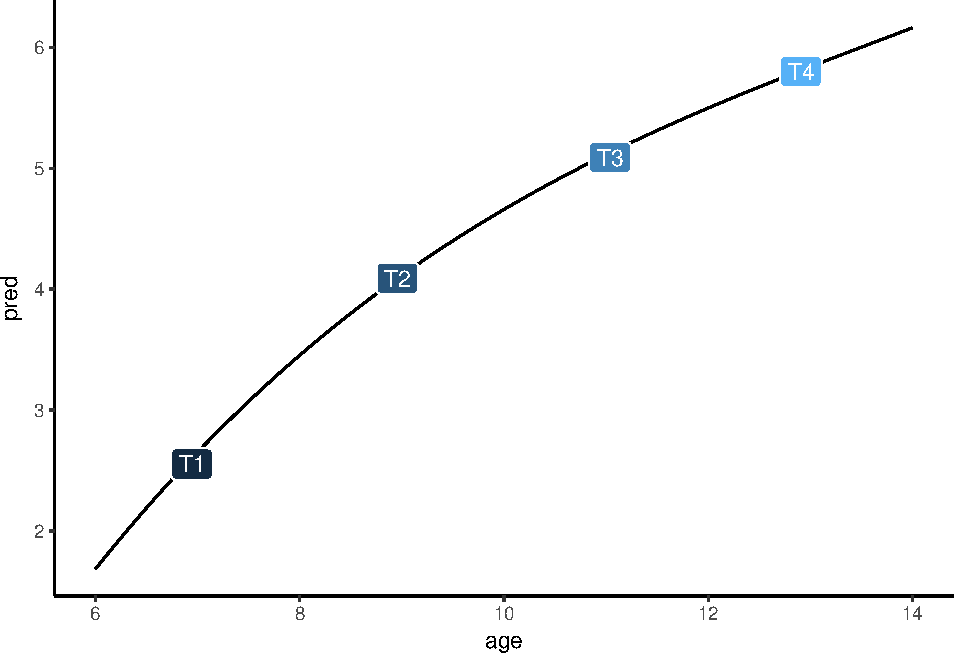
\includegraphics{Beck_HW_6_R_2_files/figure-latex/unnamed-chunk-8-1.pdf}

The plot suggests that age increased over time, such that the linear and
quadratic trends evident in both models reflect changes in age of the
sample. But as noted previously, the different scale (1,2,3,4) will
influence the size of the slopes and the intercepts.

\section{Question 6}\label{question-6}

Using Model 3, add the age of the mother (momage) as a moderator:\\
Level 1:
\(read_{ti} = \pi_{0i} + \pi_{1i}(age-10)_{ti} + \pi_{2i}(age-10)^2_{ti} + e_{ti}\)\\
Level 2: \(\pi_{0i} = \beta_{00} + \beta_{01}momage_i + r_{0i}\)\\
\(\pi_{1i} = \beta_{10} + \beta_{11}momage_i + r_{1i}\)\\
\(\pi_{2i} = \beta_{20} + \beta_{21}momage_i + r_{2i}\)

\begin{Shaded}
\begin{Highlighting}[]
\NormalTok{fit6  <-}\StringTok{ }\KeywordTok{lmer}\NormalTok{(read }\OperatorTok{~}\StringTok{  }\NormalTok{age_}\DecValTok{10}\OperatorTok{*}\NormalTok{momage }\OperatorTok{+}\StringTok{ }\NormalTok{age_10_}\DecValTok{2}\OperatorTok{*}\NormalTok{momage }\OperatorTok{+}\StringTok{ }\NormalTok{(age_}\DecValTok{10} \OperatorTok{+}\StringTok{ }\NormalTok{age_10_}\DecValTok{2} \OperatorTok{|}\StringTok{ }\NormalTok{id), }\DataTypeTok{data =}\NormalTok{ dat)}
\NormalTok{tab_}\DecValTok{6}\NormalTok{ <-}\StringTok{ }\KeywordTok{table_fun}\NormalTok{(fit6)}

\NormalTok{tab_}\DecValTok{6} \OperatorTok\StringTok{ }\KeywordTok{select}\NormalTok{(}\OperatorTok{-}\NormalTok{type) }\OperatorTok
\StringTok{  }\KeywordTok{kable}\NormalTok{(., }\StringTok{"latex"}\NormalTok{, }\DataTypeTok{escape =}\NormalTok{ F, }\DataTypeTok{digits =} \DecValTok{2}\NormalTok{, }\DataTypeTok{booktabs =}\NormalTok{ T,}
        \DataTypeTok{col.names =} \KeywordTok{c}\NormalTok{(}\StringTok{""}\NormalTok{, }\KeywordTok{c}\NormalTok{(}\StringTok{"b"}\NormalTok{, }\StringTok{"CI"}\NormalTok{))) }\OperatorTok
\StringTok{  }\KeywordTok{kable_styling}\NormalTok{(}\DataTypeTok{full_width =}\NormalTok{ F) }\OperatorTok
\StringTok{  }\KeywordTok{group_rows}\NormalTok{(}\StringTok{"Fit"}\NormalTok{, }\DecValTok{10}\NormalTok{, }\DecValTok{11}\NormalTok{) }\OperatorTok
\StringTok{  }\KeywordTok{group_rows}\NormalTok{(}\StringTok{"Fixed"}\NormalTok{, }\DecValTok{1}\NormalTok{,}\DecValTok{6}\NormalTok{) }\OperatorTok
\StringTok{  }\KeywordTok{group_rows}\NormalTok{(}\StringTok{"Random"}\NormalTok{, }\DecValTok{7}\NormalTok{, }\DecValTok{9}\NormalTok{) }\OperatorTok
\StringTok{  }\KeywordTok{add_header_above}\NormalTok{(}\KeywordTok{c}\NormalTok{(}\StringTok{" "}\NormalTok{ =}\StringTok{ }\DecValTok{1}\NormalTok{, }\StringTok{"Model 6"}\NormalTok{ =}\StringTok{ }\DecValTok{2}\NormalTok{))}
\end{Highlighting}
\end{Shaded}

\begin{table}[H]
\centering
\begin{tabular}{lll}
\toprule
\multicolumn{1}{c}{ } & \multicolumn{2}{c}{Model 6} \\
\cmidrule(l{2pt}r{2pt}){2-3}
 & b & CI\\
\midrule
\addlinespace[0.3em]
\multicolumn{3}{l}{\textbf{Fixed}}\\
\hspace{1em}Intercept & 1.41 & [-0.36, 3.13]\\
\hspace{1em}age\_10 & 0.03 & [-0.27, 0.43]\\
\hspace{1em}momage & 0.13 & [0.06, 0.19]\\
\hspace{1em}age\_10\_2 & 0.01 & [-0.07, 0.11]\\
\hspace{1em}age\_10:momage & 0.02 & [0.00, 0.03]\\
\hspace{1em}momage:age\_10\_2 & -0.00 & [-0.01, 0.00]\\
\addlinespace[0.3em]
\multicolumn{3}{l}{\textbf{Random}}\\
\hspace{1em}$\tau_{00}$ & 1.07 & [1.05, 1.37]\\
\hspace{1em}$\tau_{11}$ & 0.02 & [0.01, 0.02]\\
\hspace{1em}$\tau_{22}$ & 0.00 & [0.00, 0.00]\\
$R^2_m$ & 0.61 & \\
$R^2_c$ & 0.91 & \\
\bottomrule
\end{tabular}
\end{table}

\subsection{Part A}\label{part-a-3}

Are any of the interactions involving momage significant? If so, explain
what they mean. The interation between the linear age term and age of
the mother is significant. In other words, reading ability varies as a
function of both the age of the child and the age of the mother at
baseline. Students who are farther above the age 10 with older mothers
show steeper increases in reading age than those below age 10.

\subsection{Part B}\label{part-b-3}

Illustrate this new model by plotting the age-reading relationship
separately for mothers 1 standard deviation below the mean for momage
and 1 standard deviation above the mean for momage.

\begin{Shaded}
\begin{Highlighting}[]
\NormalTok{means <-}\StringTok{ }\NormalTok{dat }\OperatorTok\StringTok{ }\KeywordTok{summarize_at}\NormalTok{(}\KeywordTok{vars}\NormalTok{(momage), }
            \KeywordTok{funs}\NormalTok{(}\DataTypeTok{mean =} \KeywordTok{mean}\NormalTok{(., }\DataTypeTok{na.rm =}\NormalTok{ T), }
                 \DataTypeTok{sd =} \KeywordTok{sd}\NormalTok{(., }\DataTypeTok{na.rm =}\NormalTok{ T)))}

\KeywordTok{crossing}\NormalTok{(}
  \DataTypeTok{age_10 =} \KeywordTok{seq}\NormalTok{(}\OperatorTok{-}\DecValTok{4}\NormalTok{,}\DecValTok{4}\NormalTok{,.}\DecValTok{5}\NormalTok{),}
  \DataTypeTok{momage =} \KeywordTok{c}\NormalTok{(means}\OperatorTok{$}\NormalTok{mean, means}\OperatorTok{$}\NormalTok{mean }\OperatorTok{-}\StringTok{ }\NormalTok{means}\OperatorTok{$}\NormalTok{sd, means}\OperatorTok{$}\NormalTok{mean }\OperatorTok{+}\StringTok{ }\NormalTok{means}\OperatorTok{$}\NormalTok{sd)}
\NormalTok{) }\OperatorTok\StringTok{ }\KeywordTok{mutate}\NormalTok{(}\DataTypeTok{age_10_2 =}\NormalTok{ age_}\DecValTok{10}\OperatorTok{^}\DecValTok{2}\NormalTok{) }\OperatorTok
\StringTok{  }\KeywordTok{mutate}\NormalTok{(}\DataTypeTok{pred =} \KeywordTok{predict}\NormalTok{(fit6, }\DataTypeTok{newdata =}\NormalTok{ ., }\DataTypeTok{re.form =} \OtherTok{NA}\NormalTok{),}
         \DataTypeTok{momage =} \KeywordTok{mapvalues}\NormalTok{(momage, }\KeywordTok{unique}\NormalTok{(momage), }\KeywordTok{c}\NormalTok{(}\StringTok{"-1 SD"}\NormalTok{, }\StringTok{"0 SD"}\NormalTok{, }\StringTok{"+1 SD"}\NormalTok{))) }\OperatorTok

\StringTok{  }\KeywordTok{ggplot}\NormalTok{(}\KeywordTok{aes}\NormalTok{(}\DataTypeTok{x =}\NormalTok{ age_}\DecValTok{10}\NormalTok{, }\DataTypeTok{y =}\NormalTok{ pred, }\DataTypeTok{color =}\NormalTok{ momage)) }\OperatorTok{+}
\StringTok{    }\KeywordTok{geom_line}\NormalTok{(}\DataTypeTok{size =} \DecValTok{1}\NormalTok{) }\OperatorTok{+}
\StringTok{    }\KeywordTok{labs}\NormalTok{(}\DataTypeTok{x =} \StringTok{"Age Centered at 10"}\NormalTok{, }\DataTypeTok{y =} \StringTok{"Model Estimated Reading Score"}\NormalTok{, }\DataTypeTok{color =} \StringTok{"Mother Age at Baseline"}\NormalTok{) }\OperatorTok{+}
\StringTok{    }\KeywordTok{theme_classic}\NormalTok{() }\OperatorTok{+}
\StringTok{    }\KeywordTok{theme}\NormalTok{(}\DataTypeTok{legend.position =} \StringTok{"bottom"}\NormalTok{,}
          \DataTypeTok{axis.text =} \KeywordTok{element_text}\NormalTok{(}\DataTypeTok{face =} \StringTok{"bold"}\NormalTok{),}
          \DataTypeTok{axis.title =} \KeywordTok{element_text}\NormalTok{(}\DataTypeTok{face =} \StringTok{"bold"}\NormalTok{, }\DataTypeTok{size =} \KeywordTok{rel}\NormalTok{(}\FloatTok{1.2}\NormalTok{)),}
          \DataTypeTok{legend.text =} \KeywordTok{element_text}\NormalTok{(}\DataTypeTok{face =} \StringTok{"bold"}\NormalTok{),}
          \DataTypeTok{legend.title =} \KeywordTok{element_text}\NormalTok{(}\DataTypeTok{face =} \StringTok{"bold"}\NormalTok{, }\DataTypeTok{size =} \KeywordTok{rel}\NormalTok{(}\FloatTok{1.2}\NormalTok{)))}
\end{Highlighting}
\end{Shaded}

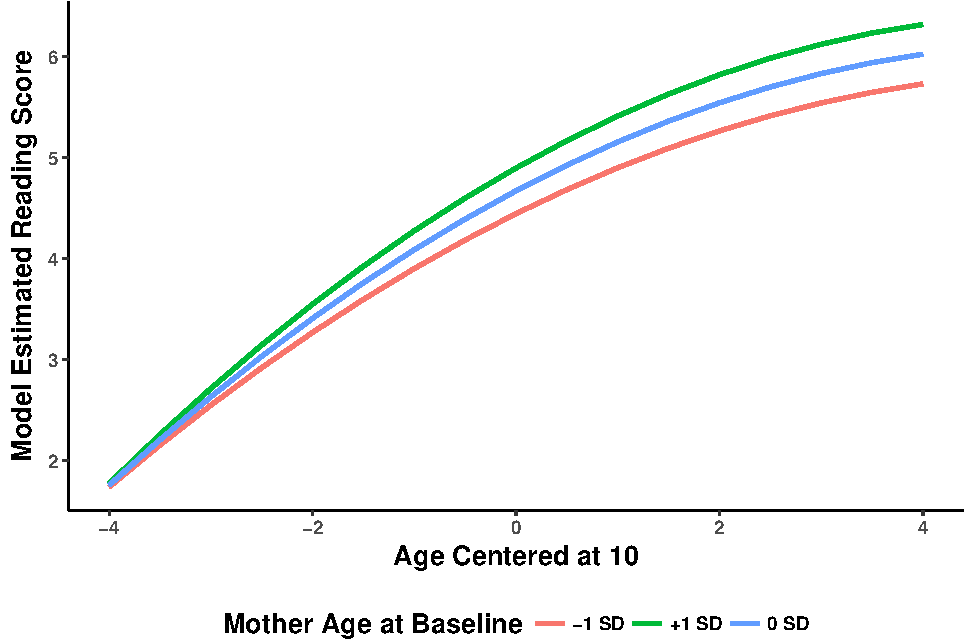
\includegraphics{Beck_HW_6_R_2_files/figure-latex/unnamed-chunk-10-1.pdf}


\end{document}
